% % % % % % % % % % % % % % % % % % % % % % % % % % % % % % % % % % % % % % % % %
% INTRO
% % % % % % % % % % % % % % % % % % % % % % % % % % % % % % % % % % % % % % % % %
\section{Time box 6}
\listoftodos
\subsection{Time box planning}

\begin{figure}[H]
	\begin{centering}
		\missingfigure{Updated timebox figure}
		%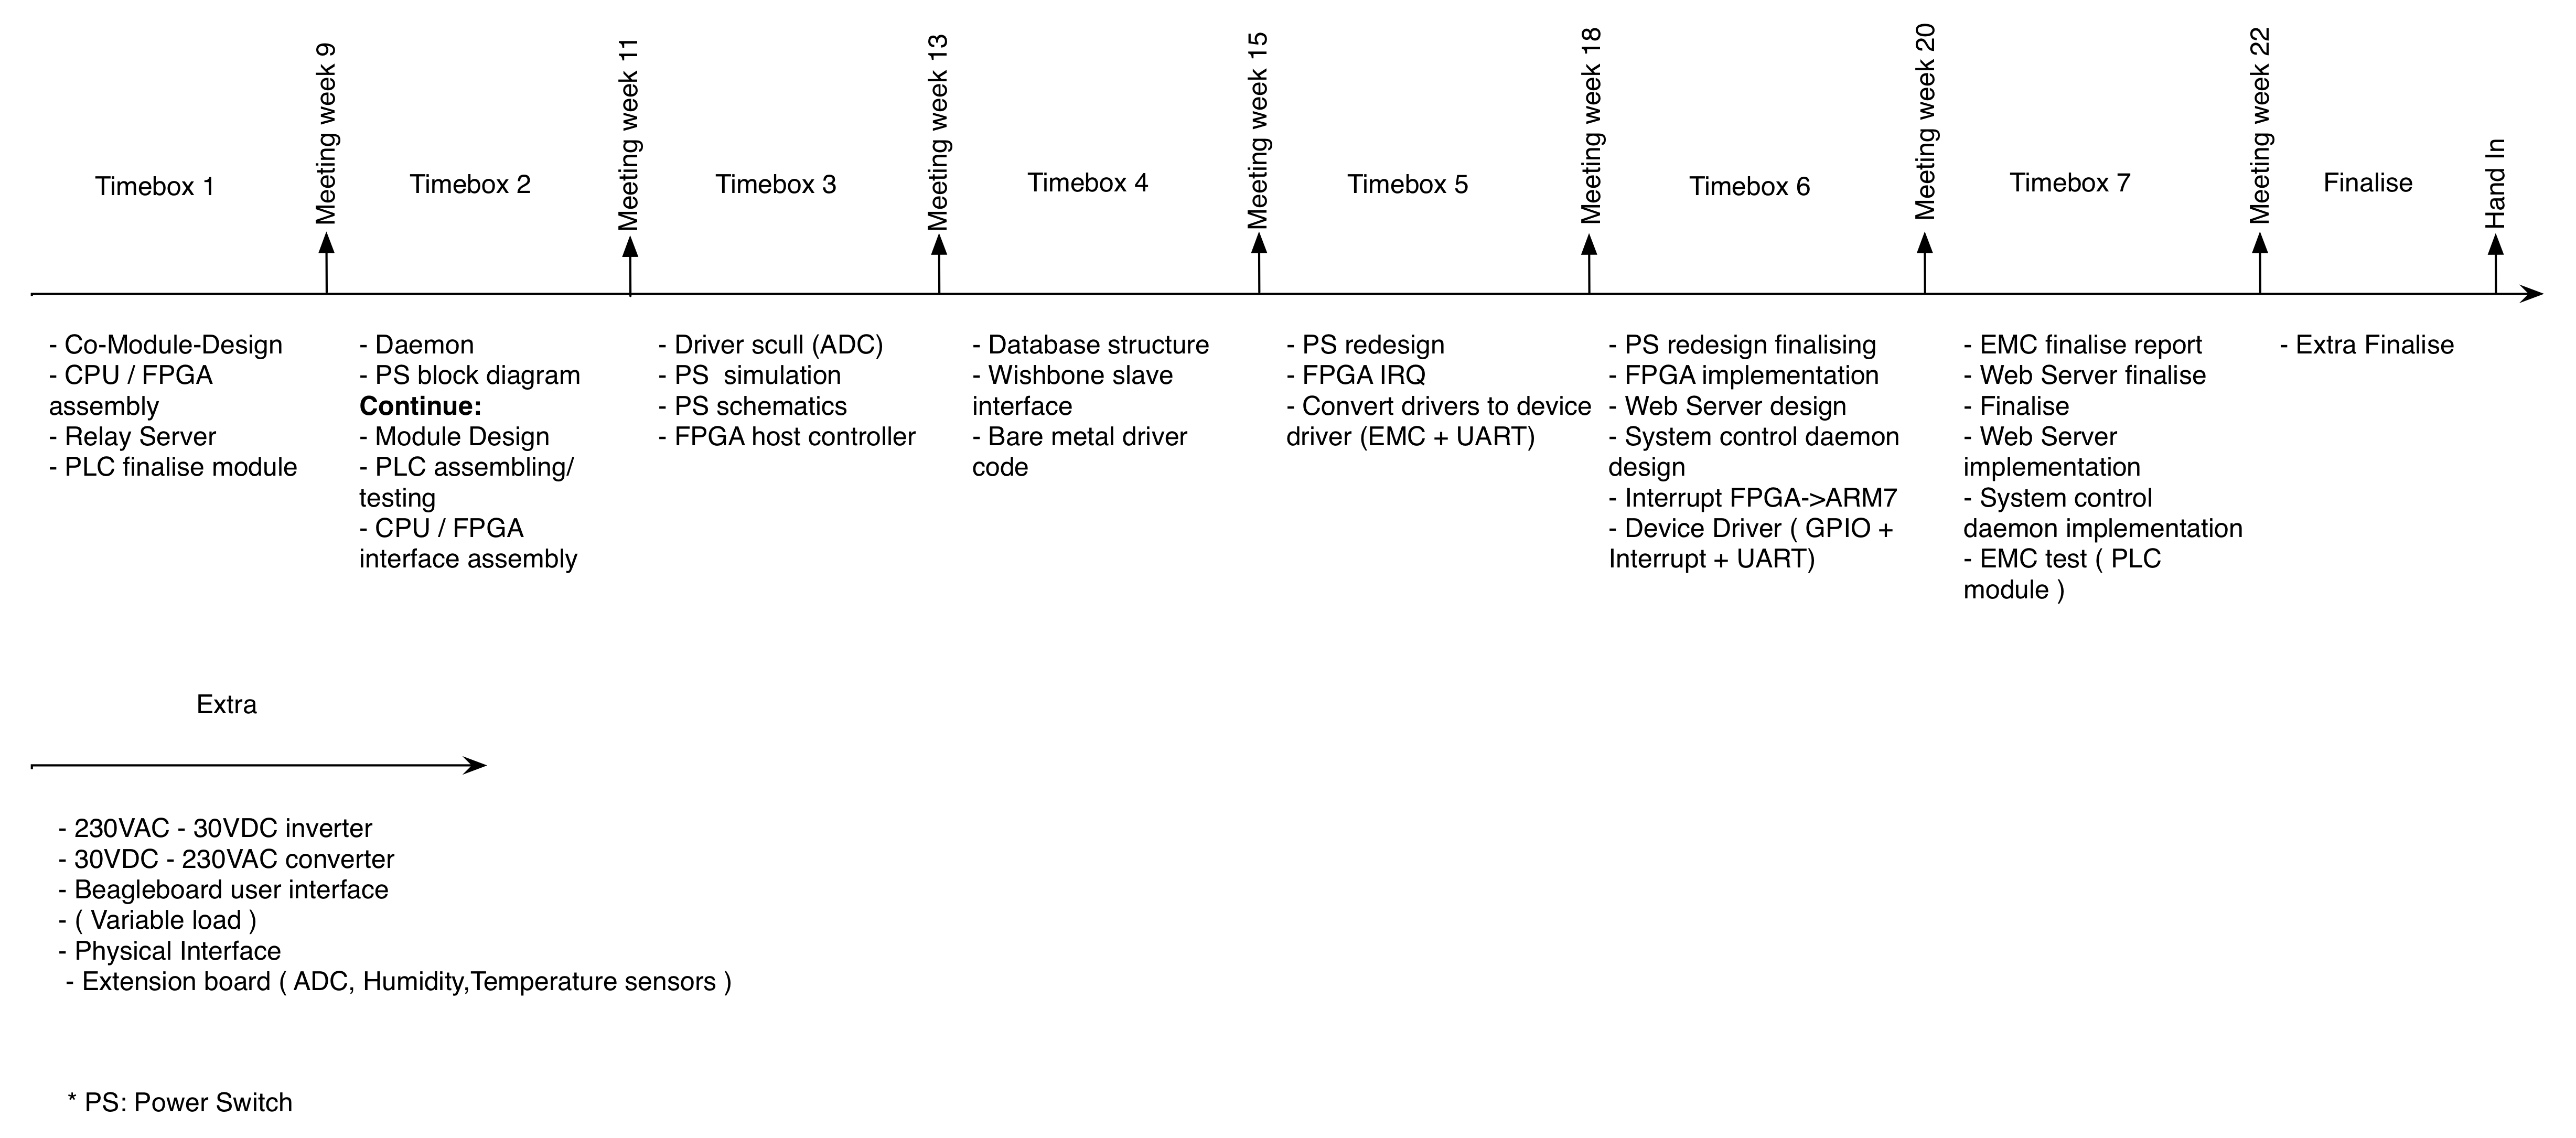
\includegraphics[width=1.0\textwidth]{images/tb_r5.png}
		%\caption{Updated time-box}
	\end{centering}
\end{figure}

\subsubsection{Work to be done in this time box}
\todo[inline]{Update List}
\begin{itemize}
	\item Theis thing
	\begin{itemize}
		\item Sub thing
	\end{itemize}
	\item Jesus thing
		\begin{itemize}
			\item sub thing
		\end{itemize}
	\item Dennis thing
	\begin{itemize}
		\item Sub thing
	\end{itemize}
\end{itemize}

\paragraph{Description:}
\todo[inline]{Update Description}
\begin{description}
	\item[Theis thing]
	\item[Jesus thing]
	\item[Dennis thing]
\end{description}

\subsubsection{Time planning}

\begin{table}[H]
\centering
	\todo[inline]{Update Time}
	\begin{tabular}{|l|c|c|c|c|c|}
		\hline
		~			& Theis thing			& Jesus thing		& Dennis thing	\\ \hline
		Estimation	& xx					& xx				& xx			\\
		Actual		& xx					& xx				& xx			\\
		Developer	& Theis					& Paulo				& Dennis		\\
		\hline
	\end{tabular}
	\caption{Estimation and actual time used on the project}
\end{table}
% % % % % % % % % % % % % % % % % % % % % % % % % % % % % % % % % % % % % % % % %
% % % % % % % % % % % % % % % % % % % % % % % % % % % % % % % % % % % % % % % % %
% Theis Thing
% % % % % % % % % % % % % % % % % % % % % % % % % % % % % % % % % % % % % % % % %
\subsection{Theis thing - Theis}
%			Intro
%					verification specification
%					deployment specification
%
\subsubsection{Analysis}
%			Analysis
%
%                Refactored block diagram
%                Refactored class diagram
%                Detailed use cases
%                User interface specification
%                System interface specification
%                Dimensioning specification 
%
\subsubsection{Design}
%       	 Design
%
%                UML/SysML deployment view(s)
%                Mechanical specifications and dimensioning
%                HW module specification per block
%                UML SW deployment view
%                Class specification
%                Refactored class diagram
%                Use case scenarios specifications
%                Sequence diagrams
%
\subsubsection{Implementation}
%     	   Implementation
%
%                Mechanical drawings with details explained
%                Electronic diagrams with details explained
%                Source code with details explained
%                Description of integration 
%
\subsubsection{Verification}
%       	 Verification
%
%                Module tests
%                Integration tests
%                Acceptance test
\subsubsection{Conclusion}
% % % % % % % % % % % % % % % % % % % % % % % % % % % % % % % % % % % % % % % % %
% % % % % % % % % % % % % % % % % % % % % % % % % % % % % % % % % % % % % % % % %
% Jesus Thing
% % % % % % % % % % % % % % % % % % % % % % % % % % % % % % % % % % % % % % % % %
\subsection{WebServer - Paulo}
%			Intro
%					verification specification
%					deployment specification
%
In time box 4 a web server was implemented at the ip address 10.1.18.223, this is a virtual machine assign as development environment for the uClinux distribution. The server is running Apache 2, PHP version 5.1.6 and MySQL server 5.0.95.
In this time box a web services system is developed for the communication between the Embedded device and the web server and the other way around. The web page made in Project 3 is incorporated with server side scripts for a fully functional web interface.
\subsubsection{Analysis}
%			Analysis
%
%                Refactored block diagram
%                Refactored class diagram
%                Detailed use cases
%                User interface specification
%                System interface specification
%                Dimensioning specification 
%
For a fully functional web interface the communication have to present in both direction since some teams need to send commands from them web page to the modules.
For the fully cooperation with all the teams a file structure was created in the server, where each team have is own folder where all the needed scripts, images and layout styles can be implemented without changing the main layout approved in project 3.
\lineparagraph{Web interface file Structure}
\begin{itemize}
	\item index.php
	\item savedata.php
	\item sendcmd.php
	\item saveip.php
	\item ajax.js
	\item login.php 
	\item cron.php 
	\item includes\/ 
	\begin{itemize}
		\item db\_connect.php
		\item db\_globals.php
	\end{itemize} 
	\item modules\/ 
		\begin{itemize}
		\item photovoltaic\/ 
			\begin{itemize}
				\item index.php
				\item db\_connect.php
				\item cron.php 
				\item (Each team choose the rest of the scripts) 
			\end{itemize}
		\item caes\/ 
			\begin{itemize}
				\item index.php 
				\item db\_connect.php 
				\item cron.php 
				\item (Each team choose the rest of the scripts) 
			\end{itemize}
		\item hub\/
			\begin{itemize} 
				\item index.php 
				\item db\_connect.php 
				\item cron.php 
				\item (Each team choose the rest of the scripts) 
			\end{itemize}
		\item battery\/ 
			\begin{itemize}
				\item index.php 
				\item db\_connect.php 
				\item cron.php 
				\item (Each team choose the rest of the scripts) 
			\end{itemize}
		\item windturbine\/ 
			\begin{itemize}
				\item index.php 
				\item db\_connect.php 
				\item cron.php 
				\item (Each team choose the rest of the scripts)
			\end{itemize}
	\end{itemize}
\end{itemize}

A short description for each script can be seen bellow:
\begin{itemize}
	\item index.php - First page of the web interface.
	\item savedata.php - Webservice that save data retrieved from the module to the database.
	\item sendcmd.php - Webservice to send commands to the desired module in the system.
	\item saveip.php - Webservice necessary to save the ip address of the energy hub, this will keep the system up and running even if a change on the network is made.
	\item ajax.js - This JavaScrit handle ajax requests when the page have no need to be reloaded, that ensure less bandwidth in the web server.
	\item login.php  - This PHP script makes the authentication of the user, creating a session when the user gives the right certifications.
	\item cron.php  - Cron jobs are running by the server in a predefined time, in this case the cron.php at the web server root will point to the cron jobs inside each module folder.
	\item db\_connect.php - Handle the connection to the MySQL server, each folder for the modules point to this file in the include folder. This way if the databse change only one file has to be changed.
	\item db\_globals.php - Includes all the global variables for the credentials to the database.
\end{itemize}

\lineparagraph{Communication}
The server have to be able to save the data retrieved from the system and send commands to the the modules connected to the energy hub. Web services are created for this functionalities.

Bellow we have the flow of the communication from the user until the final destination in this case the module or the energy hub.
\begin{figure}[H]
	\begin{centering}
		\missingfigure{Communication SendCmd.php}
		%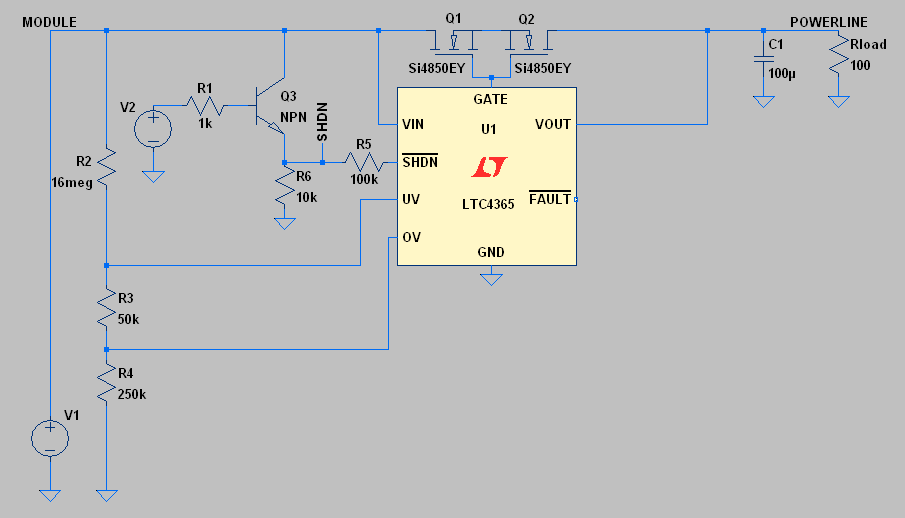
\includegraphics[width=1\textwidth]{images/tb5_LTC_simu1.png}
		%\caption{Schematics for the device LTC4365}
	\end{centering}
\end{figure}

This script doesn't give any feedback to the user, the commands send are not verified by the web server or the energy hub. The commands are handle by each module. With this system the flexibility of the system is ensured, since new modules can be added with different functionalities from the already known.
An application running in background at the energy hub uClinux, ensure that the command is translated to UART so it can be send through the power line communication to the modules.
\\\\
Measurements to be saved in the database:
\begin{figure}[H]
	\begin{centering}
		\missingfigure{Communication SendCmd.php}
		%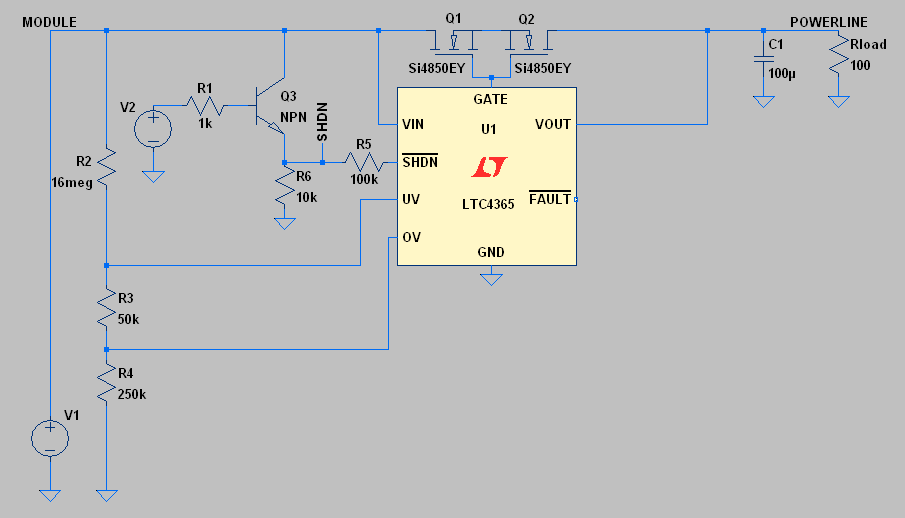
\includegraphics[width=1\textwidth]{images/tb5_LTC_simu1.png}
		%\caption{Schematics for the device LTC4365}
	\end{centering}
\end{figure}
To retrieve the measurements from the modules, an application running at the energy hub translate the data retrieved from the module through PLC to a URL request at the web server. In the server side the web server will collect the data and save it in the database.
\\\\
IP address send from the Embedded Device:
\begin{figure}[H]
	\begin{centering}
		\missingfigure{Communication SendCmd.php}
		%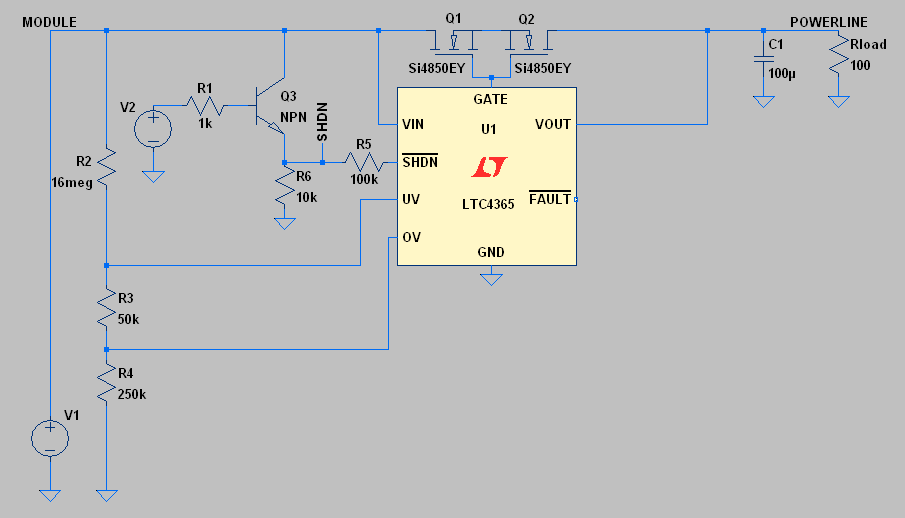
\includegraphics[width=1\textwidth]{images/tb5_LTC_simu1.png}
		%\caption{Schematics for the device LTC4365}
	\end{centering}
\end{figure}
A background application running at the uClinux, ensure that after reset the system IP address assigned by DHCP to the energy hub is saved in the database so commands can be send through the web interface.



\subsubsection{Design}
%       	 Design
%
%                UML/SysML deployment view(s)
%                Mechanical specifications and dimensioning
%                HW module specification per block
%                UML SW deployment view
%                Class specification
%                Refactored class diagram
%                Use case scenarios specifications
%                Sequence diagrams
%
\subsubsection{Implementation}
%     	   Implementation
%
%                Mechanical drawings with details explained
%                Electronic diagrams with details explained
%                Source code with details explained
%                Description of integration 
%
\subsubsection{Verification}
%       	 Verification
%
%                Module tests
%                Integration tests
%                Acceptance test
\subsubsection{Conclusion}
% % % % % % % % % % % % % % % % % % % % % % % % % % % % % % % % % % % % % % % % %
% % % % % % % % % % % % % % % % % % % % % % % % % % % % % % % % % % % % % % % % %
% Dennis Thing
% % % % % % % % % % % % % % % % % % % % % % % % % % % % % % % % % % % % % % % % %
\subsection{Dennis thing - Dennis}
%			Intro
%					verification specification
%					deployment specification
%
\subsubsection{Analysis}
%			Analysis
%
%                Refactored block diagram
%                Refactored class diagram
%                Detailed use cases
%                User interface specification
%                System interface specification
%                Dimensioning specification 
%
\subsubsection{Design}
%       	 Design
%
%                UML/SysML deployment view(s)
%                Mechanical specifications and dimensioning
%                HW module specification per block
%                UML SW deployment view
%                Class specification
%                Refactored class diagram
%                Use case scenarios specifications
%                Sequence diagrams
%
\subsubsection{Implementation}
%     	   Implementation
%
%                Mechanical drawings with details explained
%                Electronic diagrams with details explained
%                Source code with details explained
%                Description of integration 
%
\subsubsection{Verification}
%       	 Verification
%
%                Module tests
%                Integration tests
%                Acceptance test
\subsubsection{Conclusion}
% % % % % % % % % % % % % % % % % % % % % % % % % % % % % % % % % % % % % % % % %
% % % % % % % % % % % % % % % % % % % % % % % % % % % % % % % % % % % % % % % % %
% Deployment
% % % % % % % % % % % % % % % % % % % % % % % % % % % % % % % % % % % % % % % % %
\subsection{Deployment}
	%which versions of the prototype the customer will get
	%with what functionality.
\paragraph{Theis thing}
%
%
\paragraph{Jesus thing}
%
%
\paragraph{Dennis thing}
%
%